\documentclass[10pt]{article}
\usepackage[polish]{babel}
\usepackage[utf8]{inputenc}
\usepackage[T1]{fontenc}
\usepackage{graphicx}
\usepackage[export]{adjustbox}
\graphicspath{ {./images/} }
\usepackage{amsmath}
\usepackage{amsfonts}
\usepackage{amssymb}
\usepackage[version=4]{mhchem}
\usepackage{stmaryrd}
\usepackage{multirow}

\title{EGZAMIN MATURALNY Z MATEMATYKI POZIOM ROZSZERZONY }

\author{Data: 8 maja 2015 r.\\
Godzina ROZPOCZECIA: 9:00\\
CZAS PRACY: \(\mathbf{1 8 0}\) minut\\
LICZBA PUNKTÓW DO UZYSKANIA: \(\mathbf{5 0}\)}
\date{}


\begin{document}
\maketitle
\begin{center}

\includegraphics[max width=\textwidth]{2024_11_21_838c0cfd77f195c20440g-01(1)}
\end{center}



\section*{Instrukcja dla zdającego}
\begin{enumerate}
  \item Sprawdź, czy arkusz egzaminacyjny zawiera 22 strony (zadania 1-16).
\end{enumerate}

Ewentualny brak zgłoś przewodniczącemu zespołu nadzorującego egzamin.\\
2. Rozwiązania zadań i odpowiedzi wpisuj w miejscu na to przeznaczonym.\\
3. Odpowiedzi do zadań zamkniętych (1-5) przenieś na kartę odpowiedzi, zaznaczając je w części karty przeznaczonej dla zdającego. Zamaluj pola do tego przeznaczone. Błędne zaznaczenie otocz kółkiem ( \((\) ) i zaznacz właściwe.\\
4. Pamiętaj, że pominięcie argumentacji lub istotnych obliczeń w rozwiązaniu zadania otwartego (7-16) może spowodować, że za to rozwiązanie nie otrzymasz pełnej liczby punktów.\\
5. Pisz czytelnie i używaj tylko długopisu lub pióra z czarnym tuszem lub atramentem.\\
6. Nie używaj korektora, a błędne zapisy wyraźnie przekreśl.\\
7. Pamiętaj, że zapisy w brudnopisie nie będą oceniane.\\
8. Możesz korzystać z zestawu wzorów matematycznych, cyrkla i linijki oraz kalkulatora prostego.\\
9. Na tej stronie oraz na karcie odpowiedzi wpisz swój numer PESEL i przyklej naklejkę z kodem.\\
10. Nie wpisuj żadnych znaków w części przeznaczonej dla egzaminatora.\\

\includegraphics[max width=\textwidth, center]{2024_11_21_838c0cfd77f195c20440g-01}

W zadaniach od 1. do 5. wybierz i zaznacz na karcie odpowiedzi poprawna odpowiedź.

\section*{Zadanie 1. (0-1)}
Na rysunku przedstawiony jest zbiór wszystkich liczb rzeczywistych spełnających nierówność \(|2 x-8| \leq 10\).\\
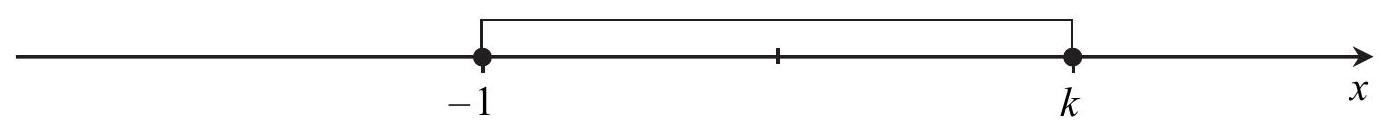
\includegraphics[max width=\textwidth, center]{2024_11_21_838c0cfd77f195c20440g-02}

Stąd wynika, że\\
A. \(k=2\)\\
B. \(k=4\)\\
C. \(k=5\)\\
D. \(k=9\)

\section*{Zadanie 2. (0-1)}
Dana jest funkcja \(f\) określona wzorem \(f(x)= \begin{cases}x-2 & \text { dla } x \leq 0 \\ |x+3|-4 \mid & \text { dla } x>0\end{cases}\)\\
Równanie \(f(x)=1\) ma dokładnie\\
A. jedno rozwiązanie.\\
B. dwa rozwiązania.\\
C. cztery rozwiązania.\\
D. pięć rozwiązań.

\section*{Zadanie 3. (0-1)}
Liczba \((3-2 \sqrt{3})^{3}\) jest równa\\
A. \(27-24 \sqrt{3}\)\\
B. \(27-30 \sqrt{3}\)\\
C. \(135-78 \sqrt{3}\)\\
D. \(135-30 \sqrt{3}\)

\section*{Zadanie 4. (0-1)}
Równanie \(2 \sin x+3 \cos x=6 \mathrm{w}\) przedziale \((0,2 \pi)\)\\
A. nie ma rozwiązań rzeczywistych.\\
B. ma dokładnie jedno rozwiązanie rzeczywiste.\\
C. ma dokładnie dwa rozwiązania rzeczywiste.\\
D. ma więcej niż dwa rozwiązania rzeczywiste.

\section*{Zadanie 5. (0-1)}
Odległość początku układu współrzędnych od prostej o równaniu \(y=2 x+4\) jest równa\\
A. \(\frac{\sqrt{5}}{5}\)\\
B. \(\frac{4 \sqrt{5}}{5}\)\\
C. \(\frac{4}{5}\)\\
D. 4

\section*{BRUDNOPIS (nie podlega ocenie)}
\begin{center}

\includegraphics[max width=\textwidth]{2024_11_21_838c0cfd77f195c20440g-03}
\end{center}

\section*{Zadanie 6. (0-2)}
Oblicz granicę \(\lim _{n \rightarrow \infty}\left(\frac{11 n^{3}+6 n+5}{6 n^{3}+1}-\frac{2 n^{2}+2 n+1}{5 n^{2}-4}\right)\). W poniższe kratki wpisz kolejno cyfrę jedności i pierwsze dwie cyfry po przecinku rozwinięcia dziesiętnego otrzymanego wyniku.\\

\includegraphics[max width=\textwidth, center]{2024_11_21_838c0cfd77f195c20440g-04}\\

\includegraphics[max width=\textwidth, center]{2024_11_21_838c0cfd77f195c20440g-04(1)}

Zadanie 7. (0-2)\\
Liczby \((-1)\) i 3 są miejscami zerowymi funkcji kwadratowej \(f\). Oblicz \(\frac{f(6)}{f(12)}\).\\

\includegraphics[max width=\textwidth, center]{2024_11_21_838c0cfd77f195c20440g-05}

Odpowiedź:

\begin{center}
\begin{tabular}{|c|l|c|c|}
\hline
\multirow{2}{*}{\begin{tabular}{c}
Wypelnia \\
egzaminator \\
\end{tabular}} & Nr zadania & \(\mathbf{6 .}\) & \(\mathbf{7 .}\) \\
\cline { 2 - 4 }
 & Maks. liczba pkt & \(\mathbf{2}\) & \(\mathbf{2}\) \\
\cline { 2 - 4 }
 & Uzyskana liczba pkt &  &  \\
\hline
\end{tabular}
\end{center}

Zadanie 8. (0-3)\\
Udowodnij, że dla każdej liczby rzeczywistej \(x\) prawdziwa jest nierówność

\[
x^{4}-x^{2}-2 x+3>0
\]

\begin{center}

\includegraphics[max width=\textwidth]{2024_11_21_838c0cfd77f195c20440g-06}
\end{center}

\begin{center}
\begin{tabular}{|c|l|c|}
\hline
\multirow{2}{*}{\begin{tabular}{l}
Wypelnia \\
egzaminator \\
\end{tabular}} & Nr zadania & 8. \\
\cline { 2 - 3 }
 & Maks. liczba pkt & 3 \\
\cline { 2 - 3 }
 & Uzyskana liczba pkt &  \\
\hline
\end{tabular}
\end{center}

\section*{Zadanie 9. (0-3)}
Dwusieczne czworokąta \(A B C D\) wpisanego w okrąg przecinają się w czterech różnych punktach: \(P, Q, R, S\) (zobacz rysunek).\\
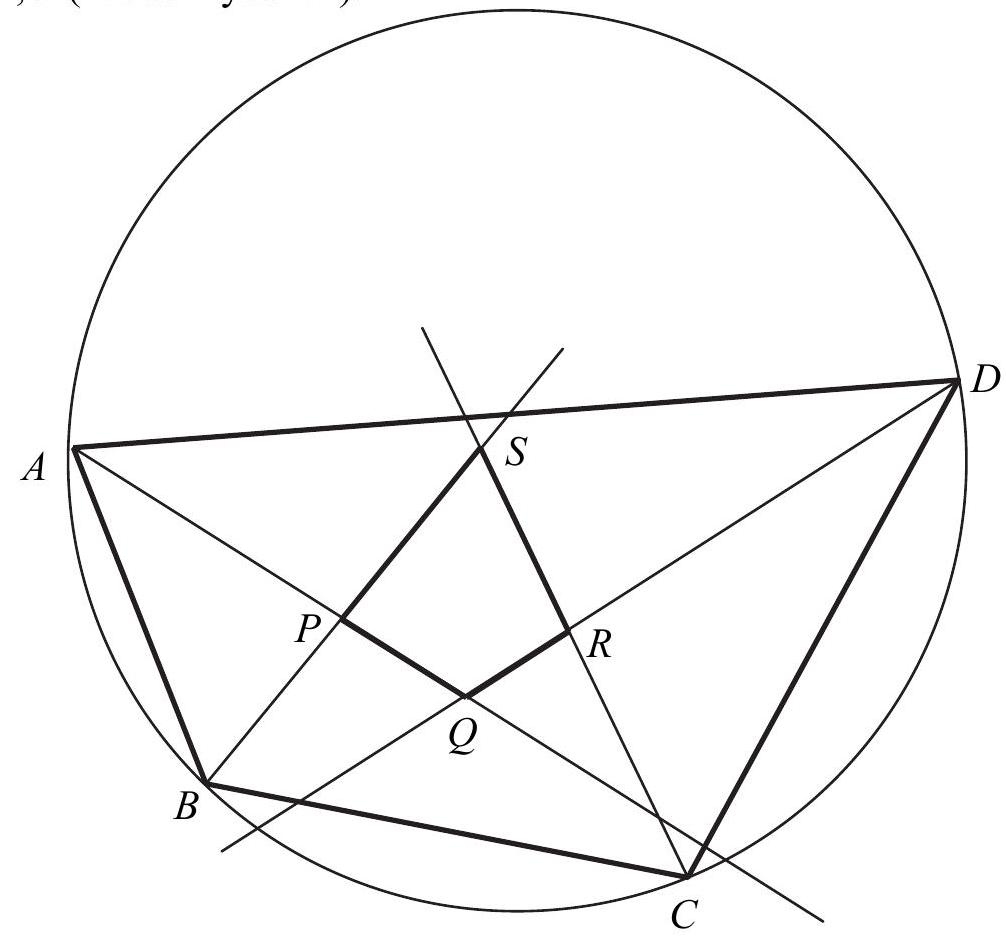
\includegraphics[max width=\textwidth, center]{2024_11_21_838c0cfd77f195c20440g-08}

Wykaż, że na czworokącie \(P Q R S\) można opisać okrąg.\\

\includegraphics[max width=\textwidth, center]{2024_11_21_838c0cfd77f195c20440g-08(1)}

\begin{center}
\begin{tabular}{|c|l|c|}
\hline
\multirow{2}{*}{\begin{tabular}{c}
Wypelnia \\
egzaminator \\
\end{tabular}} & Nr zadania & \(\mathbf{9 .}\) \\
\cline { 2 - 3 }
 & Maks. liczba pkt & \(\mathbf{3}\) \\
\cline { 2 - 3 }
 & Uzyskana liczba pkt &  \\
\hline
\end{tabular}
\end{center}

\section*{Zadanie 10. (0-4)}
Długości boków czworokąta \(A B C D\) są równe: \(|A B|=2,|B C|=3,|C D|=4,|D A|=5\). Na czworokącie \(A B C D\) opisano okrąg. Oblicz długość przekątnej \(A C\) tego czworokąta.\\

\includegraphics[max width=\textwidth, center]{2024_11_21_838c0cfd77f195c20440g-10}

Odpowiedź:

\section*{Zadanie 11. (0-4)}
W pierwszej urnie umieszczono 3 kule białe i 5 kul czarnych, a w drugiej urnie 7 kul białych i 2 kule czarne. Losujemy jedną kulę z pierwszej urny, przekładamy ją do urny drugiej i dodatkowo dokładamy do urny drugiej jeszcze dwie kule tego samego koloru, co wylosowana kula. Następnie losujemy dwie kule z urny drugiej. Oblicz prawdopodobieństwo zdarzenia polegającego na tym, że obie kule wylosowane z drugiej urny będą białe.\\

\includegraphics[max width=\textwidth, center]{2024_11_21_838c0cfd77f195c20440g-11}

Odpowiedź:

\begin{center}
\begin{tabular}{|c|l|c|c|}
\hline
\multirow{2}{*}{\begin{tabular}{c}
Wypetnia \\
egzaminator \\
\end{tabular}} & Nr zadania & 10. & 11. \\
\cline { 2 - 4 }
 & Maks. liczba pkt & 4 & 4 \\
\cline { 2 - 4 }
 & Uzyskana liczba pkt &  &  \\
\hline
\end{tabular}
\end{center}

Zadanie 12. (0-4)\\
Funkcja \(f\) określona jest wzorem \(f(x)=x^{3}-2 x^{2}+1\) dla każdej liczby rzeczywistej \(x\). Wyznacz równania tych stycznych do wykresu funkcji \(f\), które są równoległe do prostej o równaniu \(y=4 x\).

\begin{center}
\begin{tabular}{|c|c|c|c|c|c|c|c|c|c|c|c|c|c|c|c|c|c|c|c|c|c|}
\hline
 &  &  &  &  &  &  &  &  &  &  &  &  &  &  &  &  &  &  &  &  &  \\
\hline
 &  &  &  &  &  &  &  &  &  &  &  &  &  &  &  &  &  &  &  &  &  \\
\hline
 &  &  &  &  &  &  &  &  &  &  &  &  &  &  &  &  &  &  &  &  &  \\
\hline
 &  &  &  &  &  &  &  &  &  &  &  &  &  &  &  &  &  &  &  &  &  \\
\hline
 &  &  &  &  &  &  &  &  &  &  &  &  &  &  &  &  &  &  &  &  &  \\
\hline
 &  &  &  &  &  &  &  &  &  &  &  &  &  &  &  &  &  &  &  &  &  \\
\hline
 &  &  &  &  &  &  &  &  &  &  &  &  &  &  &  &  &  &  &  &  &  \\
\hline
 &  &  &  &  &  &  &  &  &  &  &  &  &  &  &  &  &  &  &  &  &  \\
\hline
 &  &  &  &  &  &  &  &  &  &  &  &  &  &  &  &  &  &  &  &  &  \\
\hline
 &  &  &  &  &  &  &  &  &  &  &  &  &  &  &  &  &  &  &  &  &  \\
\hline
 &  &  &  &  &  &  &  &  &  &  &  &  &  &  &  &  &  &  &  &  &  \\
\hline
 &  &  &  &  &  &  &  &  &  &  &  &  &  &  &  &  &  &  &  &  &  \\
\hline
 &  &  &  &  &  &  &  &  &  &  &  &  &  &  &  &  &  &  &  &  &  \\
\hline
 &  &  &  &  &  &  &  &  &  &  &  &  &  &  &  &  &  &  &  &  &  \\
\hline
 &  &  &  &  &  &  &  &  &  &  &  &  &  &  &  &  &  &  &  &  &  \\
\hline
 &  &  &  &  &  &  &  &  &  &  &  &  &  &  &  &  &  &  &  &  &  \\
\hline
 &  &  &  &  &  &  &  &  &  &  &  &  &  &  &  &  &  &  &  &  &  \\
\hline
 &  &  &  &  &  &  &  &  &  &  &  &  &  &  &  &  &  &  &  &  &  \\
\hline
 &  &  &  &  &  &  &  &  &  &  &  &  &  &  &  &  &  &  &  &  &  \\
\hline
 &  &  &  &  &  &  &  &  &  &  &  &  &  &  &  &  &  &  &  &  &  \\
\hline
 &  &  &  &  &  &  &  &  &  &  &  &  &  &  &  &  &  &  &  &  &  \\
\hline
 &  &  &  &  &  &  &  &  &  &  &  &  &  &  &  &  &  &  &  &  &  \\
\hline
 &  &  &  &  &  &  &  &  &  &  &  &  &  &  &  &  &  &  &  &  &  \\
\hline
 &  &  &  &  &  &  &  &  &  &  &  &  &  &  &  &  &  &  &  &  &  \\
\hline
 &  &  &  &  &  &  &  &  &  &  &  &  &  &  &  &  &  &  &  &  &  \\
\hline
 &  &  &  &  &  &  &  &  &  &  &  &  &  &  &  &  &  &  &  &  &  \\
\hline
 &  &  &  &  &  &  &  &  &  &  &  &  &  &  &  &  &  &  &  &  &  \\
\hline
 &  &  &  &  &  &  &  &  &  &  &  &  &  &  &  &  &  &  &  &  &  \\
\hline
 &  &  &  &  &  &  &  &  &  &  &  &  &  &  &  &  &  &  &  &  &  \\
\hline
 &  &  &  &  &  &  &  &  &  &  &  &  &  &  &  &  &  &  &  &  &  \\
\hline
 &  &  &  &  &  &  &  &  &  &  &  &  &  &  &  &  &  &  &  &  &  \\
\hline
 &  &  &  &  &  &  &  &  &  &  &  &  &  &  &  &  &  &  &  &  &  \\
\hline
 &  &  &  &  &  &  &  &  &  &  &  &  &  &  &  &  &  &  &  &  &  \\
\hline
 &  &  &  &  &  &  &  &  &  &  &  &  &  &  &  &  &  &  &  &  &  \\
\hline
 &  &  &  &  &  &  &  &  &  &  &  &  &  &  &  &  &  &  &  &  &  \\
\hline
 &  &  &  &  &  &  &  &  &  &  &  &  &  &  &  &  &  &  &  &  &  \\
\hline
 &  &  &  &  &  &  &  &  &  &  &  &  &  &  &  &  &  &  &  &  &  \\
\hline
 &  &  &  &  &  &  &  &  &  &  &  &  &  &  &  &  &  &  &  &  &  \\
\hline
 &  &  &  &  &  &  &  &  &  &  &  &  &  &  &  &  &  &  &  &  &  \\
\hline
 &  &  &  &  &  &  &  &  &  &  &  &  &  &  &  &  &  &  &  &  &  \\
\hline
 &  &  &  &  &  &  &  &  &  &  &  &  &  &  &  &  &  &  &  &  &  \\
\hline
 &  &  &  &  &  &  &  &  &  &  &  &  &  &  &  &  &  &  &  &  &  \\
\hline
 &  &  &  &  &  &  &  &  &  &  &  &  &  &  &  &  &  &  &  &  &  \\
\hline
\end{tabular}
\end{center}

\begin{center}

\includegraphics[max width=\textwidth]{2024_11_21_838c0cfd77f195c20440g-13}
\end{center}

Odpowiedź: \(\qquad\)

\begin{center}
\begin{tabular}{|c|l|c|}
\hline
\multirow{2}{*}{\begin{tabular}{c}
Wypelnia \\
egzaminator \\
\end{tabular}} & Nr zadania & 12. \\
\cline { 2 - 3 }
 & Maks. liczba pkt & 4 \\
\cline { 2 - 3 }
 & Uzyskana liczba pkt &  \\
\hline
\end{tabular}
\end{center}

\section*{Zadanie 13. (0-5)}
Dany jest trójmian kwadratowy \(f(x)=(m+1) x^{2}+2(m-2) x-m+4\). Wyznacz wszystkie wartości parametru \(m\), dla których trójmian \(f\) ma dwa różne pierwiastki rzeczywiste \(x_{1}, x_{2}\), spełniające warunek \(x_{1}^{2}-x_{2}^{2}=x_{1}^{4}-x_{2}^{4}\).\\

\includegraphics[max width=\textwidth, center]{2024_11_21_838c0cfd77f195c20440g-14}\\

\includegraphics[max width=\textwidth, center]{2024_11_21_838c0cfd77f195c20440g-15}

Odpowiedź: \(\qquad\)

\begin{center}
\begin{tabular}{|c|l|c|}
\hline
\multirow{2}{*}{\begin{tabular}{l}
Wypelnia \\
egzaminator \\
\end{tabular}} & Nr zadania & 13. \\
\cline { 2 - 3 }
 & Maks. liczba pkt & 5 \\
\cline { 2 - 3 }
 & Uzyskana liczba pkt &  \\
\hline
\end{tabular}
\end{center}

\section*{Zadanie 14. (0-5)}
Podstawą ostrosłupa \(A B C D S\) jest kwadrat \(A B C D\). Krawędź boczna \(S D\) jest wysokością ostrosłupa, a jej długość jest dwa razy większa od długości krawędzi podstawy. Oblicz sinus kąta między ścianami bocznymi \(A B S\) i \(C B S\) tego ostrosłupa.\\

\includegraphics[max width=\textwidth, center]{2024_11_21_838c0cfd77f195c20440g-16}\\

\includegraphics[max width=\textwidth, center]{2024_11_21_838c0cfd77f195c20440g-17}

Odpowiedź: \(\qquad\)

\begin{center}
\begin{tabular}{|c|l|c|}
\hline
\multirow{2}{*}{\begin{tabular}{c}
Wypelnia \\
egzaminator \\
\end{tabular}} & Nr zadania & 14. \\
\cline { 2 - 3 }
 & Maks. liczba pkt & 5 \\
\cline { 2 - 3 }
 & Uzyskana liczba pkt &  \\
\hline
\end{tabular}
\end{center}

\section*{Zadanie 15. (0-6)}
Suma wszystkich czterech współczynników wielomianu \(W(x)=x^{3}+a x^{2}+b x+c\) jest równa 0 . Trzy pierwiastki tego wielomianu tworzą ciąg arytmetyczny o różnicy równej 3 . Oblicz współczynniki \(a, b\) i \(c\). Rozważ wszystkie możliwe przypadki.\\

\includegraphics[max width=\textwidth, center]{2024_11_21_838c0cfd77f195c20440g-18}\\

\includegraphics[max width=\textwidth, center]{2024_11_21_838c0cfd77f195c20440g-19}

Odpowiedź: \(\qquad\)

\begin{center}
\begin{tabular}{|c|l|c|}
\hline
\multirow{2}{*}{\begin{tabular}{c}
Wypelnia \\
egzaminator \\
\end{tabular}} & Nr zadania & 15. \\
\cline { 2 - 3 }
 & Maks. liczba pkt & 6 \\
\cline { 2 - 3 }
 & Uzyskana liczba pkt &  \\
\hline
\end{tabular}
\end{center}

\section*{Zadanie 16. (0-7)}
Rozpatrujemy wszystkie stożki, których przekrojem osiowym jest trójkąt o obwodzie 20. Oblicz wysokość i promień podstawy tego stożka, którego objętość jest największa. Oblicz objętość tego stożka.\\

\includegraphics[max width=\textwidth, center]{2024_11_21_838c0cfd77f195c20440g-20}\\

\includegraphics[max width=\textwidth, center]{2024_11_21_838c0cfd77f195c20440g-21}

Odpowiedź:

\begin{center}
\begin{tabular}{|c|l|c|}
\hline
\multirow{2}{*}{\begin{tabular}{c}
Wypetnia \\
egzaminator \\
\end{tabular}} & Nr zadania & 16. \\
\cline { 2 - 3 }
 & Maks. liczba pkt & 7 \\
\cline { 2 - 3 }
 & Uzyskana liczba pkt &  \\
\hline
\end{tabular}
\end{center}

\section*{BRUDNOPIS (nie podlega ocenie)}

\end{document}